
\documentclass[final]{beamer}
\usepackage[ngerman]{babel}
\usepackage[utf8]{inputenc}
\usepackage[T1]{fontenc}
\usepackage{lmodern}
\usepackage{listings}
\usepackage{graphicx}
\usepackage{xcolor}
\newcommand{\ThemeFolder}{fsibeamertheme}
\RequirePackage{\ThemeFolder/beamerthemeFSI}

\DeclareGraphicsExtensions{.pdf,.png}

\mode<presentation>

\title{PO-Briefing}

\setbeamertemplate{title page}{
	\begin{center}
		\color{FSIblue}
			\resizebox{\textwidth}{!}{PO-Briefing}\\
			\vspace{0.3\baselineskip}
		\tableofcontents
	\end{center}
}

\begin{document}

\begin{frame}
	\titlepage
\end{frame}

\section{Prüfungsanmeldung}
\begin{frame}
\frametitle{Prüfungsanmeldung - Wann?}
\begin{itemize}

\item Sommersemester: 			Anfang Juni
\item Wintersemester: 				Anfang Dezember

\item Erinnerung per Mail
\end{itemize}

\end{frame}

\begin{frame}
\frametitle{Prüfungsanmeldung - Wo?}
\begin{itemize}
\item \url{https://qis2.hs-karlsruhe.de}
	\begin{itemize}
		\item Prüfungsverwaltung
		\item Prüfungsan- und -abmeldung
	\end{itemize}
\end{itemize}
	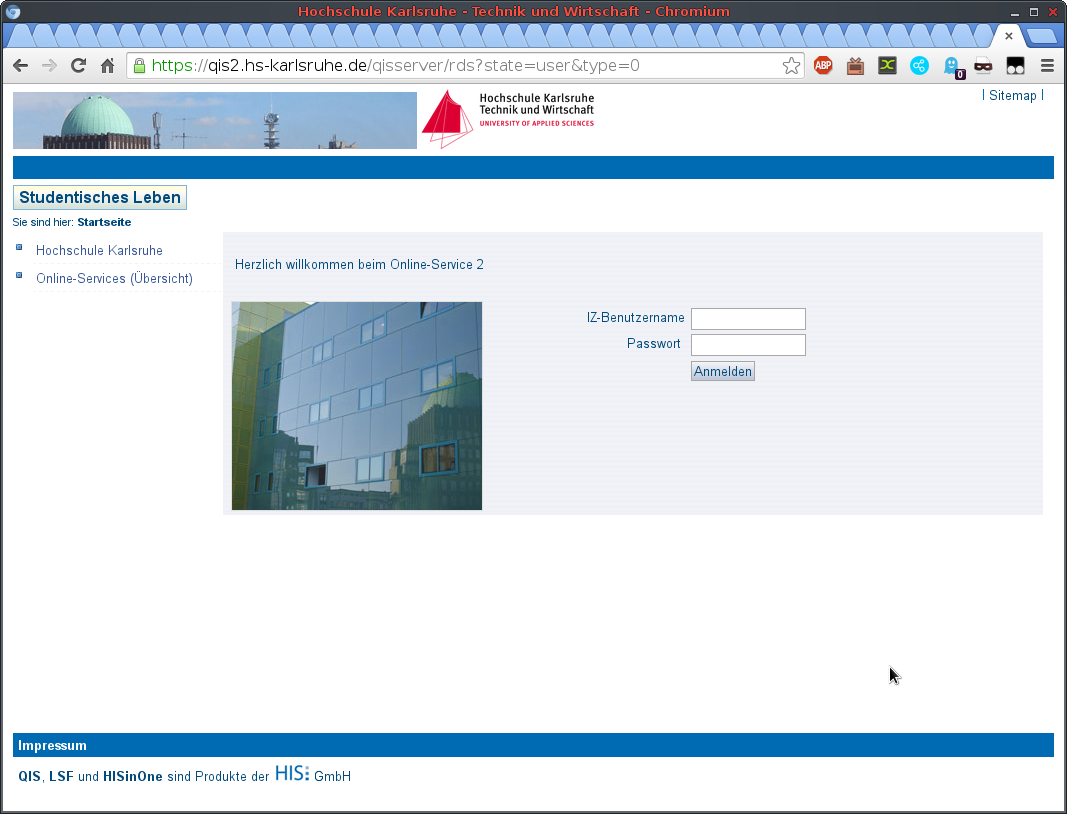
\includegraphics[scale=0.3]{qis.png}
\end{frame}

\begin{frame}
\frametitle{Prüfungsanmeldung - Was?}
\begin{itemize}
	\item Alle Vorlesungen, die ihr schreiben wollt und Labore, die ihr gemacht habt.
	\item Man ist bereits für alle Klausuren laut Prüfungsordnung angemeldet.
	\item Wahlpflichtfächer und Extrafächer müssen angemeldet werden.
	\item Immer überprüfen!!!
\end{itemize}
\end{frame}

\begin{frame}
\frametitle{Prüfungsabmeldung}
\begin{itemize}
\item \url{https://qis2.hs-karlsruhe.de}
\item Mindestens ein voller Kalendertag zwischen Prüfung und Abmeldung.
\item Nichterscheinen: Durchgefallen (5.0)
\item Zwei mal schieben möglich.
\item Nicht möglich, falls Wiederholungsprüfung.
\end{itemize}
\end{frame}

\section{Laboranmeldungen}
\begin{frame}
\frametitle{Laboranmeldungen}
	\begin{itemize}
	\item Von Labor zu Labor unterschiedlich:
		\begin{itemize}
		\item https://ilias.hs-karlsruhe.de
		\item Listen vor dem Sekretariat
		\item …
		\end{itemize}
	\end{itemize}
\end{frame}

\section{Grundstudium}
\begin{frame}
\frametitle{Grundstudium}
\begin{itemize}
	\item Die ersten zwei Semester sind Grundstudium.
	\item Die Noten aus diesen Klausuren zählen NICHT ins Bachelorzeugnis.
	\item Zum Abschluss: Bachelorvorzeugnis
\end{itemize}
\end{frame}

\section{Fragen}
\begin{frame}
\frametitle{Fragen?}
\begin{center}
\url{www.hska.info}\\
\url{www.hska.info/faq}\\
\vspace{.5cm}
\url{chat.hska.info}\\
(\#fsi auf irc.freenode.net)
\end{center}
\end{frame}
\end{document}
